\chapter{The TCP Models}
\label{cha:tcp}


\section{Overview}

TCP protocol is the most widely used protocol of the Internet. It provides
reliable, ordered delivery of stream of bytes from one application on one computer
to another application on another computer. It is used by such applications as
World Wide Web, email, file transfer amongst others.

The baseline TCP protocol is described in RFC793, but other tens of RFCs
contains modifications and extensions to the TCP. These proposals
enhance the efficiency and safety of the TCP protocol and they are widely
implemented in the real TCP modules. As a result, TCP is a complex protocol
and sometimes it is hard to see how the different requirements interacts
with each other.

The TCP modules of the INET framework implements the following RFCs:

\begin{tabular}{ll}
RFC 793 & Transmission Control Protocol \\
RFC 896 & Congestion Control in IP/TCP Internetworks \\
RFC 1122 & Requirements for Internet Hosts -- Communication Layers \\
RFC 1323 & TCP Extensions for High Performance \\ 
RFC 2018 & TCP Selective Acknowledgment Options \\
RFC 2581 & TCP Congestion Control \\
RFC 2883 & An Extension to the Selective Acknowledgement (SACK) Option for TCP \\
RFC 3042 & Enhancing TCP's Loss Recovery Using Limited Transmit \\
RFC 3390 & Increasing TCP's Initial Window \\
RFC 3517 & A Conservative Selective Acknowledgment (SACK)-based Loss Recovery \newline
                 Algorithm for TCP \\
RFC 3782 & The NewReno Modification to TCP's Fast Recovery Algorithm \\
\end{tabular}

In this section we describe the features of the TCP protocol specified by these RFCs,
the following sections deal with the implementation of the TCP in the INET framework. 

\subsection{TCP segments}

The TCP module transmits a stream of the data over the unreliable, datagram service 
that the IP layer provides. When the application writes a chunk of data into the socket,
the TCP module breaks it down to packets and hands it over the IP. On the receiver side,
it collects the recieved packets, order them, and acknowledges the reception. The packets
that are not acknowledged in time are retransmitted by the sender.

The TCP procotol can address each byte of the data stream by \emph{sequence numbers}.
The sequence number is a 32-bit unsigned integer, if the end of its range is reached,
it is wrapped around.

The layout of the TCP segments is described in RFC793:

\begin{center}
\begin{bytefield}{32}
\bitheader{0,3,4,7,8,15,16,31} \\
\bitbox{16}{Source Port} &
\bitbox{16}{Destination Port} \\
\bitbox{32}{Sequence Number} \\
\bitbox{32}{Acknowledgment Number} \\
\bitbox{4}{\small Data Offset} &
\bitbox{6}{Reserved} &
\bitbox{6}{Flags} &
\bitbox{16}{Window} \\
\bitbox{16}{Checksum} &
\bitbox{16}{Urgent Pointer} \\
\bitbox{24}{Options} &
\bitbox{8}{Padding} \\
\wordbox{3}{Data}
\end{bytefield}
\end{center}

Here
\begin{itemize}
  \item the Source and Destination Ports, together with the Source and Destination
  addresses of the IP header identifies the communication endpoints.
  \item the Sequence Number identifier of the first data byte transmitted in the sequence,
  Sequence Number + 1 identifies the second byte, so on. If the SYN flag is set it consumes
  one sequence number before the data bytes.
  \item the Acknowlegment Number refers to the next byte (if the ACK flag is set) expected
  by the receiver using its sequence number
  \item the Data Offset is the length of the TCP header in 32-bit words (needed because the
  Options field has variable length)
  \item the Reserved bits are unused
  \item the Flags field composed of 6 bits:
  \begin{itemize}
    \item URG: Urgent Pointer field is significant
    \item ACK: Acknowledgment field is significant
    \item PSH: Push Function
    \item RST: Reset the connection
    \item SYN: Synchronize sequence number
    \item FIN: No more data from sender
  \end{itemize}
  \item the Window is the number of bytes the receiver TCP can accept (because of its
  limited buffer)
  \item the Checksum is the 1-complement sum of the 16-bit words of the IP/TCP header and
  data bytes
  \item the Urgent Pointer is the offset of the urgent data (if URG flag is set)
  \item the Options field is variable length, it can occupy 0-40 bytes in the header and is
  always padded to a multiple of 4 bytes.
\end{itemize}

\subsection{TCP connections}

When two applications are communicating via TCP, one of the applications is the client,
the other is the server. The server usually starts a socket with a well known local port
and waits until a request comes from clients. The client applications are issue connection
requests to the port and address of the service they want to use.

After the connection is established both the client and the server can send and receive data.
When no more data is to be sent, the application closes the socket. The application can still
receive data from the other direction. The connection is closed when both communication partner
closed its socket.

...

When opening the connection an initial sequence number is choosen and communicated to the
other TCP in the SYN segment. This sequence number can not be a constant value (e.g. 0),
because then data segments from a previous incarnation of the connection (i.e. a connection
with same addresses and ports) could be erronously accepted in this connection. Therefore
most TCP implementation choose the initial sequence number according to the system clock.


\begin{figure}
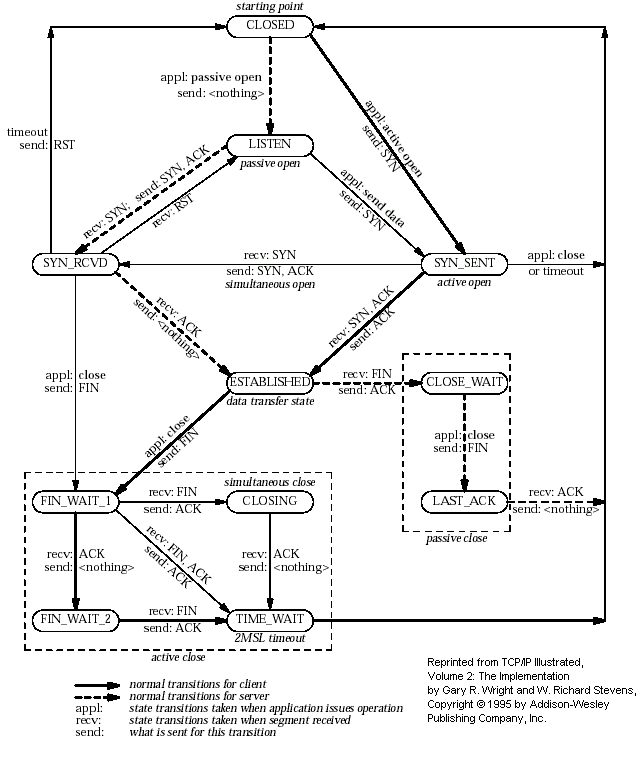
\includegraphics[width=\textwidth]{figures/tcpstate}
\caption{TCP state diagram}
\label{fig:tcp_states}
\end{figure}

\subsection{Flow control}
\label{subsec:flow_control}

The TCP module of the receiver buffers the data of incoming segments.
This buffer has a limited capacity, so it is desirable to notify the sender
about how much data the client can accept. The sender stops the transmission
if this space exhausted.

In TCP every ACK segment holds a Window field; this is the available space
in the receiver buffer. When the sender reads the Window, it can send at most
Window unacknowledged bytes.

\subsubsection*{Window Scale option}

% RFC1323
The TCP segment contains a 16-bit field for the Window, thus allowing at most
65535 byte windows. If the network bandwidth and latency is large, it is surely
too small. The sender should be able to send bandwitdh*latency bytes without
receiving ACKs. 

For this purpose the Window Scale (WS) option had been introduced in RFC1323.
This option specifies a scale factor used to interpret the value of the Window field.
The format is the option is:

\begin{center}
\begin{bytefield}{24}
\bitbox{8}{Kind=3} &
\bitbox{8}{Length=3} &
\bitbox{8}{shift.cnt}
\end{bytefield}
\end{center}

If the TCP want to enable window sizes greater than 65535, it should send
a WS option in the SYN segment or SYN/ACK segment (if received a SYN with WS
option). Both sides must send the option in the SYN segment to enable window scaling,
but the scale in one direction might differ from the scale in the other direction.
The $shift.cnt$ field is the 2-base logarithm of the window scale of the sender.
Valid values of $shift.cnt$ are in the $[0,14]$ range.

\subsubsection*{Persistence timer}

When the reciever buffer is full, it sends a 0 length window in the ACK segment
to stop the sender. Later if the application reads the data,
it will repeat the last ACK with an updated window to resume data sending.
If this ACK segment is lost, then the sender is not notified, so a deadlock
happens.

To avoid this situation the sender starts a Persistence Timer when it received
a 0 size window. If the timer expires before the window is increased it send
a probe segment with 1 byte of data. It will receive the current window of the
receiver in the response to this segment.

\subsubsection*{Keepalive timer}

TCP keepalive timer is used to detect dead connections.

\subsection{Transmission policies}
\label{subsec:trans_policies}

\subsubsection*{Retransmissions}

% source: RFC1222 4.3.2.1 and Tannenbaum 6.5.10

When the sender TCP sends a TCP segment it starts a
retransmission timer.
If the ACK arrives before the timer expires it is stopped,
otherwise it triggers a retransmission of the segment.

If the retransmission timeout (RTO) is too high, then lost segments
causes high delays, if it is too low, then the receiver gets
too many useless duplicated segments. For optimal behaviour, the
timeout must be dynamically determined.

Jacobson suggested to measure the RTT mean and deviation
and apply the timeout:

$$ RTO = RTT + 4 * D $$

Here RTT and D are the measured smoothed roundtrip time and its
smoothed mean deviation. They are initialized to 0 and updated each time an
ACK segment received according to the following formulas:

$$ RTT = \alpha*RTT + (1-\alpha) * M $$

$$ D = \alpha*D + (1-\alpha)*|RTT-M| $$

where $M$ is the time between the segments send and the acknowledgment
arrival. Here the $\alpha$ smoothing factor is typically $7/8$.

One problem may occur when computing the round trip: if the
retransmission timer timed out and the segment is sent again,
then it is unclear that the received ACK is a response to the
first transmission or to the second one. To avoid confusing the
RTT calculation, the segments that have been retransmitted
do not update the RTT. This is known as Karn's modification.
He also suggested to double the $RTO$ on each failure until the
segments gets through (``exponential backoff'').

\subsubsection*{Delayed ACK algorithm}

% RFC1122 4.2.3.2

A host that is receiving a stream of TCP data segments can
increase efficiency in both the Internet and the hosts by
sending fewer than one ACK (acknowledgment) segment per data
segment received; this is known as a "delayed ACK" [TCP:5].

Delay is max. 500ms.

A delayed ACK gives the application an opportunity to
update the window and perhaps to send an immediate
response.  In particular, in the case of character-mode
remote login, a delayed ACK can reduce the number of
segments sent by the server by a factor of 3 (ACK,
window update, and echo character all combined in one
segment).

In addition, on some large multi-user hosts, a delayed
ACK can substantially reduce protocol processing
overhead by reducing the total number of packets to be
processed [TCP:5].  However, excessive delays on ACK's
can disturb the round-trip timing and packet "clocking"
algorithms [TCP:7].

% RFC2581 3.2

a TCP receiver SHOULD send an immediate ACK
when the incoming segment fills in all or part of a gap in the
sequence space.

\subsubsection*{Nagle's algorithm}

RFC896 describes the ``small packet problem": when the application
sends single-byte messages to the TCP, and it transmitted immediatly
in a 41 byte TCP/IP packet (20 bytes IP header, 20 bytes TCP header,
1 byte payload), the result is a 4000\% overhead that can cause
congestion in the network.

The solution to this problem is to delay the transmission until
enough data received from the application and send all collected
data in one packet. Nagle proposed that
when a TCP connection has outstanding data that has not
yet been acknowledged, small segments should not be sent
until the outstanding data is acknowledged.

\subsubsection*{Silly window avoidance}

The Silly Window Syndrome (SWS) is described in RFC813. It occurs when
a TCP receiver advertises a small window and the TCP sender immediately
sends data to fill the window. Let's take the example when the sender
process writes a file into the TCP stream in big chunks, while the
receiver process reads the bytes one by one. The first few bytes
are transmitted as whole segments until the receiver buffer
becomes full. Then the application reads one
byte, and a window size 1 is offered to the sender. The sender sends
a segment with 1 byte payload immediately, the receiver buffer becomes
full, and after reading 1 byte, the offered window is 1 byte again.
Thus almost the whole file is transmitted in very small segments.

In order to avoid SWS, both sender and receiver must try to avoid this
situation. The receiver must not advertise small windows and the sender
must not send small segments when only a small window is advertised.

In RFC813 it is offered that
\begin{enumerate}
  \item the receiver should not advertise windows that is smaller than the maximum
        segment size of the connection
  \item the sender should wait until the window is large enough for a maximum sized
        segment. 
\end{enumerate}

\subsubsection*{Timestamp option}

Efficient retransmissions depends on precious RTT measurements.
Packet losses can reduce the precision of these measurements radically.
When a segment lost, the ACKs received in that window can not be used;
thus reducing the sample rate to one RTT data per window. This is
unacceptable if the window is large.

The proposed solution to the problem is to use a separate timestamp
field to connect the request and the response on the sender side.
The timestamp is transmitted as a TCP option. The option contains two
32-bit timestamps:

\begin{center}
\begin{bytefield}{80}
\bitbox{8}{Kind=5} &
\bitbox{8}{Length=10} &
\bitbox{32}{TS Value} &
\bitbox{32}{TS Echo Reply} &
\end{bytefield}
\end{center}

Here the TS Value (TSVal) field is the current value of the timestamp
clock of the TCP sending the option, TS Echo Reply (TSecr) field is
0 or echoes the timestamp value of that was sent by the remote TCP.
The TSscr field is valid only in ACK segments that acknowledges new
data. Both parties should send the TS option in their SYN segment
in order to allow the TS option in data segments.

The timestamp option can also be used for PAWS (protection against wrapped
sequence numbers).


\subsection{Congestion control}

Flow control allows the sender to slow down the transmission when the
receiver can not accept them because of memory limitations. However
there are other situations when a slow down is desirable. If the sender
transmits a lot of data into the network it can overload the processing
capacities of the network nodes, so packets are lost in the network
layer.

For this purpose another window is maintained at the sender side, the
congestion window (CWND). The congestion window is a sender-side limit
on the amount of data the sender can transmit into the network before
receiving ACK. More precisely, the sender can send at most max(CWND, WND)
bytes above SND.UNA, therefore $ SND.NXT < SND.UNA + max(CWND, WND) $ is
guaranteed.

The size of the congestion window is dinamically determined by monitoring
the state of the network.

% RFC2581
% 
% Definitions:
% SMSS: sender maximum segment size
% RMSS: receiver maximum segment size (default 536)
% rwnd: most recently advertised receiver window
% IW: initial sender's congestion window
% LW: loss window, size of congestion window after a TCP sender detects loss
% RW: restart window, size of congestion window after a TCP restarts transmission after an idle period
% fligth size: amount of data has been sent but not yet acknowledged
% cwnd: congestion window, sender-size limit on the amount of data the sender
%       can transmit into the network before receiving an ACK
% rwnd: receiver advertised window, receiver-side limit on the amount of outstanding data
% sstresh: whether slow start or congestion avoidance used
% 
% IW <= 2*MSS


\subsubsection*{Slow Start and Congestion Avoidance}

There are two algorithm that updates the congestion window, ``Slow Start''
and ``Congestion Avoidance''. They are specified in RFC2581.

\begin{pseudocode}
$cwnd \gets 2*SMSS$
$ssthresh \gets $ upper bound of the window (e.g. $65536$)
whenever ACK received
  if $cwnd < ssthresh$
    $cwnd \gets cwnd + SMSS$
  otherwise
    $cwnd \gets cwnd + SMSS*SMSS/cwnd$
whenever packet loss detected
  $cwnd \gets SMSS$
  $ssthresh \gets max(FlightSize/2, 2*SMSS)$
\end{pseudocode}

Slow Start means that when the connection opened the sender initially
sends the data with a low rate. This means that the initial
window (IW) is at most 2 MSS, but no more than 2 segments. If there was no packet loss,
then the congestion window is increased rapidly, it is doubled in each flight.
When a packet loss is detected, the congestion window is reset to 1 MSS (loss window, LW)
and the ``Slow Start'' is applied again.

\begin{note}
RFC3390 increased the IW to roughly 4K bytes: $min(4*MSS, max(2*MSS, 4380))$.
\end{note}

When the congestion window reaches a certain limit (slow start threshold),
the ``Congestion Avoidance'' algorithm is applied. During ``Congestion Avoidance''
the window is incremented by 1 MSS per round-trip-time (RTT). This is usually
implemented by updating the window according to the $ cwnd += SMSS*SMSS/cwnd $
formula on every non-duplicate ACK.

The Slow Start Threshold is updated when a packet loss is detected.
It is set to $max(FlightSize/2, 2*SMSS)$.

How the sender estimates the flight size? The data sent, but not yet acknowledged.

How the sender detect packet loss? Retransmission timer expired.


\subsubsection*{Fast Retransmit and Fast Recovery}

RFC2581 specifies two additional methods to increase the efficiency
of congestion control: ``Fast Retransmit'' and ``Fast Recovery''.

``Fast Retransmit'' requires that the receiver signal the event,
when an out-of-order segment arrives. It is achieved by sending
an immediate duplicate ACK. The receiver also sends an immediate
ACK when the incoming segment fills in a gap or part of a gap.

When the sender receives the duplicated ACK it knows that some
segment after that sequence number is received out-of-order or
that the network duplicated the ACK. If 3 duplicated ACK received
then it is more likely that a segment was dropped or delayed.
In this case the sender starts to retransmit the segments
immediately.

``Fast Recovery'' means that ``Slow Start'' is not applied
when the loss is detected as 3 duplicate ACKs. The arrival
of the duplicate ACKs indicates that the network is not fully
congested, segments after the lost segment arrived, as well
the ACKs.

% Details?
% 
%    1.  When the third duplicate ACK is received, set ssthresh to no more
%        than the value given in equation 3.
% 
%    2.  Retransmit the lost segment and set cwnd to ssthresh plus 3*SMSS.
%        This artificially "inflates" the congestion window by the number
%        of segments (three) that have left the network and which the
%        receiver has buffered.
% 
%    3.  For each additional duplicate ACK received, increment cwnd by
%        SMSS.  This artificially inflates the congestion window in order
%        to reflect the additional segment that has left the network.
% 
%    4.  Transmit a segment, if allowed by the new value of cwnd and the
%        receiver's advertised window.
% 
%    5.  When the next ACK arrives that acknowledges new data, set cwnd to
%        ssthresh (the value set in step 1).  This is termed "deflating"
%        the window.
% 
%        This ACK should be the acknowledgment elicited by the
%        retransmission from step 1, one RTT after the retransmission
%        (though it may arrive sooner in the presence of significant out-
%        of-order delivery of data segments at the receiver).
%        Additionally, this ACK should acknowledge all the intermediate
%        segments sent between the lost segment and the receipt of the
%        third duplicate ACK, if none of these were lost.

\subsubsection*{Loss Recovery Using Limited Transmit}

If there is not enough data to be send after a lost segment,
then the Fast Retransmit algorithm is not activated, but the
costly retranmission timeout used.

RFC3042 suggests that the sender TCP should send a new data segment
in response to each of the first two duplicate acknowledgement. Transmitting
these segments increases the probability that TCP can recover from a single
lost segment using the fast retransmit algorithm, rather than using a costly
retransmission timeout.

\subsubsection*{Selective Acknowledgments}

% RFC2018

With selective
acknowledgments (SACK), the data receiver can inform the sender about all
segments that have arrived successfully, so the sender need
retransmit only the segments that have actually been lost.

With the help of this information the sender can detect
\begin{itemize}
  \item replication by the network
  \item false retransmit due to reordering
  \item retransmit timeout due to ACK loss
  \item early retransmit timeout
\end{itemize}


In the congestion control algorithms described so far 
the sender has only rudimentary information about which
segments arrived at the receiver. On the other hand
the algorithms are implemented completely on the sender side,
they only require that the client sends immediate ACKs on
duplicate segments. Therefore they can work in a heterogenous
environment, e.g. a client with Tahoe TCP can communicate with
a NewReno server. On the other hand SACK must be supported by
both endpoint of the connection to be used.

If a TCP supports SACK it includes the \emph{SACK-Permitted} option
in the SYN/SYN-ACK segment when initiating the connection.
The SACK extension enabled for the connection if the \emph{SACK-Permitted}
option was sent and received by both ends. The option occupies
2 octets in the TCP header:

\begin{center}
\begin{bytefield}{16}
\bitbox{8}{Kind=4} &
\bitbox{8}{Length=2}
\end{bytefield}
\end{center}

If the SACK is enabled then the data receiver adds SACK option
to the ACK segments. The SACK option informs the sender about
non-contiguous blocks of data that have been received and queued.
The meaning of the \emph{Acknowledgement Number} is unchanged,
it is still the cumulative sequence number. Octets received
before the \emph{Acknowledgement Number} are kept by the receiver,
and can be deleted from the sender's buffer. However the receiver
is allowed to drop the segments that was only reported in the SACK
option.

The \emph{SACK} option contains the following fields:

\begin{center}
\begin{bytefield}{32}
\bitbox[]{16}{} &
\bitbox{8}{Kind=5} &
\bitbox{8}{Length} \\
\bitbox{32}{Left Edge of 1st Block} \\
\bitbox{32}{Right Edge of 1st Block} \\
\wordbox[]{1}{$\vdots$ \\[1ex]} \\
\bitbox{32}{Left Edge of nth Block} \\
\bitbox{32}{Right Edge of nth Block}
\end{bytefield}
\end{center}

Each block represents received bytes of data that are
contiguous and isolated with one exception: if a segment
received that was already ACKed (i.e. below $RCV.NXT$),
it is included as the first block of the \emph{SACK} option.
The purpose is to inform the sender about a spurious retransmission.

Each block in the option occupies 8 octets. The TCP header
allows 40 bytes for options, so at most 4 blocks can be
reported in the \emph{SACK} option (or 3 if TS option is also used).
The first block is used for reporting the most recently received
data, the following blocks repeats the most recently reported
SACK blocks. This way each segment is reported at least 3 times,
so the sender receives the information even if some ACK segment is
lost.


\textbf{SACK based loss recovery}

% RFC3517: loss recovery based on SACK

Now lets see how the sender can use the information in the
\emph{SACK} option. First notice that it can give a better
estimation of the amount of data outstanding in the network
(called $pipe$ in RFC3517).
If $highACK$ is the highest ACKed sequence number, and
$highData$ of the highest sequence number transmitted,
then the bytes between $highACK$ and $highData$ can be
in the network. However $ pipe \neq highData - highACK $
if there are lost and retransmitted segments:

$$ pipe = highData - highACK - lostBytes + retransmittedBytes $$

A segment is supposed to be lost if it was not received
but 3 segments recevied that comes after this segment in the sequence
number space.
This condition is detected by the sender by receiving
either 3 discontiguous SACKed blocks, or at least
$3*SMSS$ SACKed bytes above the sequence numbers of the
lost segment.

The transmission of data starts with a \emph{Slow Start} phase.
If the loss is detected by 3 duplicate ACK, the sender
goes into the recovery state: it sets
$cwnd$ and $ssthresh$ to $FlightSize / 2$.
It also remembers the $highData$ variable, because
the recovery state is left when this sequence number
is acknowledged.

In the recovery state it sends data
until there is space in the congestion window (i.e. $cwnd-pipe >= 1 SMSS$)
The data of the segment is choosen by the following rules (first rule that applies):

\begin{enumerate}
  \item send segments that is lost and not yet retransmitted
  \item send segments that is not yet transmitted
  \item send segments that is not yet retransmitted and possibly fills a gap
        (there is SACKed data above it)
\end{enumerate}

If there is no data to send, then the sender waits for the next ACK, updates
its variables based on the data of the received ACK, and then try to transmit
according to the above rules.

If an RTO occurs, the sender drops the collected SACK information and
initiates a Slow Start. This is to avoid a deadlock when the receiver
dropped a previously SACKed segment.

% highACK: highest ACKed sequence number
% 
% highData: highest sequence number transmitted
% 
% highRxt: highest sequence number which has been retransmitted
% 
% 
% Normal phase: before the first loss, until 3 duplicate ACK
% 
% Loss recovery phase: until ACK for RecoveryPoint received
% 
% On the transition to loss recovery phase
% \begin{enumerate}
%   \item RecoveryPoint=HighData
%   \item ssthresh=cwnd=FlightSize/2
%   \item compute \emph{pipe}
% \end{enumerate}
% 
% In the loss recovery phase, for each incoming ACK:
% 
% \begin{enumerate}
%   %\Alph
%   \item if cumulative ACK above RecoveryPoint, leave loss recovery phase
%   \item update SACK info and compute pipe
%   \item if $cwnd-pipe >= 1 SMSS$ send one or more segments (if there is data to send)
%   \item update HighRxt, HighData according to the sent bytes
%   \item increment $pipe$ by the amount of data sent
%   \item if $cwnd-pipe >= 1 SMSS$, continue sending
% \end{enumerate}
% 
% Which bytes to be send are determined as follows:
% 
% \begin{enumerate}
%   \item if there is a byte which is lost and not yet retransmitted, send that in 1 segment
%   \item otherwise if there is unsent data, send that in 1 segment
%   \item otherwise if there is not yet retransmitted data, and above that there is SACKed data, send that
%   \item otherwise there is no data to send
% \end{enumerate}


\section{TCP module}

The \nedtype{TCP} simple module is the main implementation of the TCP protocol in the INET framework.
Other implementation are described in section \ref{sec:other_tcp}.
The \nedtype{TCP} module as other transport protocols work above the network layer and below the application
layer, therefore it has gates to be connected with the IPv4 or IPv6 network (ipIn/ipOut or ipv6In/ipv6Out),
and with the applications (appIn[k], appOut[k]).
One \nedtype{TCP} module can serve several application modules, and several
connections per application. The $k$th application connects to \nedtype{TCP}'s
\ttt{appIn[k]} and \ttt{appOut[k]} ports. 

The TCP module usually specified by its module interface
(\nedtype{ITCP}) in the NED definition of hosts, so it can be replaced with any implementation
that communicates through the same gates. The \nedtype{TCP} model relies on
sending and receiving \cppclass{IPControlInfo} objects
attached to TCP segment objects as control info (see \ffunc{cMessage::setControlInfo()}).

The \nedtype{TCP} module manages several \cppclass{TCPConnection} object each
holding the state of one connection. The connections are identified
by a connection identifier which is choosen by the application.
If the connection is established it can also be identified by
the local and remote addresses and ports. The TCP module simply
dispatches the incoming application commands and packets to
the corresponding object.

\subsection{TCP packets}
\label{subsec:tcp_packets}

The INET framework models the TCP header with the \msgtype{TCPSegment} message class.
This contains the fields of a TCP frame, except:
\begin{compactitem}
  \item \emph{Data Offset}: represented by \ffunc{cMessage::length()}
  \item \emph{Reserved}
  \item \emph{Checksum}: modelled by \ffunc{cMessage::hasBitError()}
  \item \emph{Options}: only EOL, NOP, MSS, WS, SACK\_PERMITTED, SACK and TS are possible
  \item \emph{Padding}
\end{compactitem}

The Data field can either be represented by (see \cppclass{TCPDataTransferMode}):
\begin{compactitem}
  \item encapsulated C++ packet objects,
  \item raw bytes as a \cppclass{ByteArray} instance,
  \item its byte count only,
\end{compactitem}
corresponding to transfer modes OBJECT, BYTESTREAM, BYTECOUNT resp.


\subsection{TCP commands}

The application and the TCP module communicates with each other
by sending \cppclass{cMessage} objects. These messages are specified
in the \ffilename{TCPCommand.msg} file.

The \cppclass{TCPCommandCode} enumeration defines the message kinds
that are sent by the application to the TCP:
\begin{itemize}
  \item TCP\_C\_OPEN\_ACTIVE: active open
  \item TCP\_C\_OPEN\_PASSIVE: passive open
  \item TCP\_C\_SEND: send data
  \item TCP\_C\_CLOSE: no more data to send
  \item TCP\_C\_ABORT: abort connection
  \item TCP\_C\_STATUS: request status info from TCP
\end{itemize}

Each command message should have an attached control info of type \cppclass{TCPCommand}.
Some commands (TCP\_C\_OPEN\_xxx, TCP\_C\_SEND) use subclasses.
The \cppclass{TCPCommand} object has a \fvar{connId} field that identifies the
connection locally within the application. \fvar{connId} is to be chosen by the
application in the open command.

When the application receives a message from the TCP, the message kind is
set to one of the \cppclass{TCPStatusInd} values:
\begin{itemize}
  \item TCP\_I\_ESTABLISHED: connection established
  \item TCP\_I\_CONNECTION\_REFUSED: connection refused
  \item TCP\_I\_CONNECTION\_RESET: connection reset
  \item TCP\_I\_TIME\_OUT: connection establish timer went off, or max retransmission count reached
  \item TCP\_I\_DATA: data packet
  \item TCP\_I\_URGENT\_DATA: urgent data packet
  \item TCP\_I\_PEER\_CLOSED: FIN received from remote TCP
  \item TCP\_I\_CLOSED: connection closed normally
  \item TCP\_I\_STATUS: status info
\end{itemize}

These messages also have an attached control info with \cppclass{TCPCommand}
or derived type (TCPConnectInfo, TCPStatusInfo, TCPErrorInfo).

% receive() calls are not modeled, incoming data passed to the application right away
% how accurate the modeling of the receiver window?

\subsection{TCP parameters}

The \nedtype{TCP} module has the following parameters:
\begin{itemize}
  \item \fpar{advertisedWindow} in bytes, corresponds with the maximal receiver buffer capacity (Note: normally, NIC queues should be at least this size, default is  14*mss)
  \item \fpar{delayedAcksEnabled} delayed ACK algorithm (RFC 1122) enabled/disabled
  \item \fpar{nagleEnabled} Nagle's algorithm (RFC 896) enabled/disabled
  \item \fpar{limitedTransmitEnabled} Limited Transmit algorithm (RFC 3042) enabled/disabled (can be used for TCPReno/TCPTahoe/TCPNewReno/TCPNoCongestionControl)
  \item \fpar{increasedIWEnabled} Increased Initial Window (RFC 3390) enabled/disabled
  \item \fpar{sackSupport} Selective Acknowledgment (RFC 2018, 2883, 3517) support (header option) (SACK will be enabled for a connection if both endpoints support it)
  \item \fpar{windowScalingSupport} Window Scale (RFC 1323) support (header option) (WS will be enabled for a connection if both endpoints support it)
  \item \fpar{timestampSupport} Timestamps (RFC 1323) support (header option) (TS will be enabled for a connection if both endpoints support it)
  \item \fpar{mss} Maximum Segment Size (RFC 793) (header option, default is 536)
  \item \fpar{tcpAlgorithmClass} the name of TCP flavour
  
             Possible values are ``TCPReno'' (default), ``TCPNewReno'', ``TCPTahoe'', ``TCPNoCongestionControl'' and ``DumpTCP''.
             In the future, other classes can be written which implement Vegas, LinuxTCP  or other variants.
             See section \ref{sec:tcp_algorithms} for detailed description of implemented flavours.

             Note that TCPOpenCommand allows tcpAlgorithmClass to be chosen per-connection.

  \item \fpar{recordStats} if set to false it disables writing excessive amount of output vectors
\end{itemize}

\subsection{Statistics}

The \nedtype{TCP} module collects the following vectors:

\begin{tabular}{l p{10cm}}
  \ttt{send window} & $SND.WND$ \\
  \ttt{receive window} & $RCV.WND$, after SWS avoidance applied \\
  \ttt{advertised window} & $RCV.NXT + RCV.WND$ \\
  \ttt{sent seq} & \emph{Sequence Number} of the sent segment \\
  \ttt{sent ack} & \emph{Acknowledgement Number} of the sent segment \\
  \ttt{rcvd seq} & \emph{Sequence Number} of the received segment \\
  \ttt{rcvd ack} & \emph{Acknowledgement Number} of the received segment \\
  \ttt{unacked bytes} & number of sent and unacknowledged bytes ($max of SND.NXT - SND.UNA$) \\
  \ttt{rcvd dupAcks} & number of duplicate acknowledgements, reset to 0 when $SND.UNA$ advances \\
  \ttt{pipe} & the value of the SACK $pipe$ variable
               (estimated number of bytes outstanding in the network) \\
  \ttt{sent sacks} & number of SACK blocks sent \\
  \ttt{rcvd sacks} & number of SACK blocks received \\
  \ttt{rcvd oooseg} & number of received out-of-order segments \\
  \ttt{rcvd naseg} & number of received unacceptable segments (outside the receive window) \\
  \ttt{rcvd sackedBytes} & total amount of SACKed bytes in the buffer of the sender \\
  \ttt{tcpRcvQueueBytes} & number of bytes in the receiver's buffer \\
  \ttt{tcpRcvQueueDrops} & number of bytes dropped by the receiver (not enough buffer) \\
  \ttt{cwnd} & congestion window \\
  \ttt{ssthresh} & slow start threshold \\
  \ttt{measured RTT} & measured round trip time \\
  \ttt{smoothed RTT} & smoothed round trip time \\
  \ttt{RTTVAR} & measured smoothed variance of round trip time \\
  \ttt{RTO} & retransmission timeout \\
  \ttt{numRTOs} & number of retransmission timeouts occured \\
\end{tabular}

If the \fpar{recordStats} parameter is set to \fkeyword{false}, then none
of these output vectors are generated.

% \subsection{Animation effects}
% 
% TCP module text: number of connections sorted by state
% 
% log, log verbose

\section{TCP connections}

Most part of the TCP specification is implemented in the
\cppclass{TCPConnection} class: takes care of the state machine,
stores the state variables (TCB), sends/receives SYN, FIN, RST, ACKs, etc. 
TCPConnection itself implements the basic TCP ``machinery'', 
the details of congestion control are factored out to
\cppclass{TCPAlgorithm} classes.

There are two additional objects the \cppclass{TCPConnection}
relies on internally: instances of \cppclass{TCPSendQueue} and
\cppclass{TCPReceiveQueue}. These polymorph classes manage the actual data stream,
so \cppclass{TCPConnection} itself only works with sequence number variables.
This makes it possible to easily accomodate need for various types of
simulated data transfer: real byte stream, "virtual" bytes (byte counts
only), and sequence of \cppclass{cMessage} objects (where every message object is
mapped to a TCP sequence number range).

\subsection{Opening connections}

Applications can open a local port for incoming connections by sending
the TCP a TCP\_C\_PASSIVE\_OPEN message. The attached control info
(an \cppclass{TCPOpenCommand}) contains the local address and port.
The application can specify that it wants to handle
only one connection at a time, or multiple simultanous connections. If the
\fvar{fork} field is true, it emulates the Unix accept(2) semantics: a new
connection structure is created for the connection (with a new \fvar{connId}),
and the connection with the old connection id remains listening.
If \fvar{fork} is false, then the first connection is accepted
(with the original \fvar{connId}),
and further incoming connections will be refused by the TCP by sending an RST segment.
The \fvar{dataTransferMode} field in \cppclass{TCPOpenCommand} specifies
whether the application data is transmitted as C++ objects, real bytes or byte
counts only. The congestion control algorithm can also be specified
on a per connection basis by setting \fvar{tcpAlgorithmClass} field to the
name of the algorithm.

The application opens a connection to a remote server by sending the TCP
a TCP\_C\_OPEN\_ACTIVE command. The TCP creates a \cppclass{TCPConnection}
object an sends a SYN segment. The initial sequence number selected according
to the simulation time: 0 at time 0, and increased by 1 in each 4$\mu$s.
If there is no response to the SYN segment, it retry after 3s, 9s, 21s and
45s. After 75s a connection establishment timeout (TCP\_I\_TIMEOUT) reported
to the application and the connection is closed.

When the connection gets established, TCP sends a TCP\_I\_ESTABLISHED
notification to the application. The attached control info
(a \cppclass{TCPConnectInfo} instance)
will contain the local and remote addresses and ports of the connection.
If the connection is refused by the remote peer (e.g. the port is not open),
then the application receives a TCP\_I\_CONNECTION\_REFUSED message.

\begin{note}
If you do active OPEN, then send data and close before the connection
has reached ESTABLISHED, the connection will go from SYN\_SENT to CLOSED
without actually sending the buffered data. This is consistent with
RFC 793 but may not be what you would expect.
\end{note}

\begin{note}
Handling segments with SYN+FIN bits set (esp. with data too) is
inconsistent across TCPs, so check this one if it is of importance.
\end{note}

\subsection{Sending Data}

The application can write data into the connection
by sending a message with TCP\_C\_SEND kind to the TCP.
The attached control info must be of type \cppclass{TCPSendCommand}.

The TCP will add the message to the \emph{send queue}.
As mentioned in section \ref{subsec:tcp_packets}, there are three methods
to represent the application data in the TCP segment.
Consequently there are three type of send queues.
 
If the payload is transmitted as a message
object, then \cppclass{TCPMsgBasedSendQueue};
if the payload is a byte array then \cppclass{TCPDataStreamSendQueue};
if only the message lengths are represented then \cppclass{TCPVirtualDataSendQueue}
are the classes of send queues. The appropriate queue is created based
on the value of the \fpar{dataTransferMode} parameter of the Open command, no
further configuration is needed.

The message is handed over to the IP when there is
enough room in the windows. If Nagle's algorithm is
enabled, the TCP will collect 1 SMSS data and sends
them toghether.

\begin{note}
There is no way to set the PUSH and URGENT flags, when sending data.
\end{note}

% FIXME urgBit is never set
% FIXME model TCP_NODELAY, there is no PUSH flag in socket.send() (TCP_PUSH option ?)

\subsection{Receiving Data}

The TCP connection stores the incoming segments in the
\emph{receive queue}. The receive queue also has three flavours:
\cppclass{TCPMsgBasedRcvQueue}, \cppclass{TCPDataStreamRcvQueue}
and \cppclass{TCPVirtualDataRcvQueue}. The queue is created
when the connection is opened according to the \fvar{dataTransferMode}
of the connection.

Finite receive buffer size is modeled by the \fpar{advertisedWindow}
parameter. If receive buffer is exhausted (by out-of-order
segments) and the payload length of a new received segment
is higher than the free receiver buffer, the new segment will be dropped.
Such drops are recorded in \emph{tcpRcvQueueDrops} vector.

If the \emph{Sequence Number} of the received segment is the next
expected one, then the data is passed
to the application immediately. The \ffunc{recv()} call of
Unix is not modeled.

The data of the segment, which can be either a \cppclass{cMessage}
object, a \cppclass{ByteArray} object, or a simply byte count,
is passed to the application in a message that has
TCP\_I\_DATA kind.

% when the cMessage object is passed to the app? when last byte received?

\begin{note}
The TCP module does not handle the segments with PUSH or URGENT
flags specially. The data of the segment passed to the application
as soon as possible, but the application can not find out if that
data is urgent or pushed.
\end{note}

\subsection{RESET handling}

When an error occures at the TCP level, an RST segment is sent to
the communication partner and the connection is aborted.
Such error can be:
\begin{compactitem}
  \item arrival of a segment in CLOSED state
  \item an incoming segment acknowledges something not yet sent.
\end{compactitem}

The receiver of the RST it will abort the connection.
If the connection is not yet established, then the passive
end will go back to the LISTEN state and waits for another
incoming connection instead of aborting.    

\subsection{Closing connections}

When the application does not have more data to send, it closes the
connection by sending a TCP\_C\_CLOSE command to the TCP. The TCP
will transmit all data from its buffer and in the last segment sets
the FIN flag. If the FIN is not acknowledged in time it will be
retransmitted with exponential backoff.

The TCP receiving a FIN segment will notify the application that
there is no more data from the communication partner. It sends
a TCP\_I\_PEER\_CLOSED message to the application containing
the connection identifier in the control info.

When both parties have closed the connection, the applications
receive a TCP\_I\_CLOSED message and the connection object is
deleted. (Actually one of the TCPs waits for $2 MSL$ before
deleting the connection, so it is not possible to reconnect
with the same addresses and port numbers immediately.)

\subsection{Aborting connections}

The application can also abort the connection. This means that
it does not wait for incoming data, but drops the data associated
with the connection immediately. For this purpose the application
sends a TCP\_C\_ABORT message specifying the connection identifier
in the attached control info. The TCP will send a RST to the
communication partner and deletes the connection object. The application
should not reconnect with the same local and remote addresses and
ports within MSL (maximum segment lifetime), because segments
from the old connection might be accepted in the new one.

\subsection{Status Requests}

Applications can get detailed status information about an existing
connection. For this purpose they send the TCP module a TCP\_C\_STATUS
message attaching an \cppclass{TCPCommand} info with the identifier
of the connection. The TCP will respond with a TCP\_I\_STATUS message
with a \cppclass{TCPStatusInfo} attachement. This control info
contains the current state, local and remote addresses and ports,
the initial sequence numbers, windows of the receiver and sender, etc.

% \section{TCP queues}
% 
% Three queues belong to each TCP connection. The \emph{send queue} holds
% the segments not yet transmitted or not yet acknowledged. 
% The \emph{receive queue} holds the segments received by the TCP,
% but not yet passed to the application. (This happens only when the segment
% is received out-of-order.). The \emph{retransmit queue} holds additional
% information about the segments in the send queue.
% 
% As mentioned in section \ref{subsec:tcp_packets}, there are three methods
% to represent the application data in the TCP segment. Consequently the above
% queues comes in three flavours. If the payload is transmitted as a message
% object, then \cppclass{TCPMsgBasedRcvQueue} and \cppclass{TCPMsgBasedSendQueue};
% if the payload is a byte array then \cppclass{TCPDataStreamRcvQueue} and
% \cppclass{TCPDataStreamSendQueue}; if only the message lengths are represented
% then \cppclass{TCPVirtualDataRcvQueue} and \cppclass{TCPVirtualDataSendQueue}
% are the classes of receive/send queues. The appropriate queue is created based
% on the value of the \fpar{dataTransferMode} parameter of the Open command, no
% further configuration is needed. The retransmit queue is always an
% instance of \cppclass{TCPSACKRexmitQueue}.
% 
% The interfaces of the receive/send queues are defined by the
% \cppclass{TCPReceiveQueue} and \cppclass{TCPSendQueue} classes.
% 
% % mapping segments into the sequence space
% 

\section{TCP algorithms}
\label{sec:tcp_algorithms}

The \cppclass{TCPAlgorithm} object controls
retransmissions, congestion control and ACK sending: delayed acks, slow start,
fast retransmit, etc. They are all extends the \cppclass{TCPAlgorithm} class.
This simplifies the design of \cppclass{TCPConnection} and makes it a lot easier to
implement TCP variations such as Tahoe, NewReno, Vegas or LinuxTCP.

Currently implemented algorithm classes are \cppclass{TCPReno},
\cppclass{TCPTahoe}, \cppclass{TCPNewReno}, \cppclass{TCPNoCongestionControl}
and \cppclass{DumbTCP}. It is also possible to add new TCP variations
by implementing \cppclass{TCPAlgorithm}.

\includegraphics{figures/tcp_algorithms}

The concrete TCP algorithm class to use can be chosen per connection (in OPEN)
or in a module parameter.

\subsection{DumbTCP}

A very-very basic \cppclass{TCPAlgorithm} implementation, with hardcoded
retransmission timeout (2 seconds) and no other sophistication. It can be
used to demonstrate what happened if there was no adaptive
timeout calculation, delayed acks, silly window avoidance,
congestion control, etc. Because this algorithm does not
send duplicate ACKs when receives out-of-order segments,
it does not work well together with other algorithms.

\subsection{TCPBaseAlg}

The \cppclass{TCPBaseAlg} is the base class of the INET implementation
of Tahoe, Reno and New Reno. It implements basic TCP
algorithms for adaptive retransmissions, persistence timers,
delayed ACKs, Nagle's algorithm, Increased Initial Window
-- EXCLUDING congestion control. Congestion control
is implemented in subclasses.

\subsubsection*{Delayed ACK}

When the \fpar{delayedAcksEnabled} parameter is set to \fkeyword{true},
\cppclass{TCPBaseAlg} applies a 200ms delay before sending ACKs.

\subsubsection*{Nagle's algorithm}

When the \fpar{nagleEnabled} parameter is \fkeyword{true}, then
the algorithm does not send small segments if there is outstanding
data. See also \ref{subsec:trans_policies}.

\subsubsection*{Persistence Timer}

The algorithm implements \emph{Persistence Timer} (see \ref{subsec:flow_control}).
When a zero-sized window is received it starts the timer with 5s timeout.
If the timer expires before the window is increased, a 1-byte probe is
sent. Further probes are sent after 5, 6, 12, 24, 48, 60, 60, 60, ...
seconds until the window becomes positive.

\subsubsection*{Initial Congestion Window} 

Congestion window is set to 1 SMSS when the connection is established.
If the \fpar{increasedIWEnabled} parameter is true, then the initial
window is increased to 4380 bytes, but at least 2 SMSS and at most 4 SMSS.
The congestion window is not updated afterwards; subclasses can
add congestion control by redefining virtual methods of the
\cppclass{TCPBaseAlg} class.

\subsubsection*{Duplicate ACKs}

The algorithm sends a duplicate ACK when an out-of-order
segment is received or when the incoming segment fills in all
or part of a gap in the sequence space.

\subsubsection*{RTO calculation}

Retransmission timeout ($RTO$) is calculated according to
Jacobson algorithm (with $\alpha=7/8$), and Karn's modification is also applied.
The initial value of the $RTO$ is 3s, its minimum is 1s,
maximum is 240s (2 MSL).

% FIXME according to RFC1222, MIN_REXMIT_TIMEOUT should be a fraction of second
%       to accomodate high speed LANs. In the linux kernel (net/tcp.h)
%       TCP_RTO_MIN is HZ/5 = 200ms. Consider 0ms lower bound.

\subsection{TCPNoCongestion}

TCP with no congestion control (i.e. congestion window kept very large).
Can be used to demonstrate effect of lack of congestion control.

% FIXME 65536 is not 'very large' nowadays, with window scaling
%       the receive window can be as large as 2^30 bytes.
%       Consequently the initial ssthresh is too small for Tahoe/Reno/NewReno,
%       Slow Start is stopped too early first time.

\subsection{TCPTahoe}

The \cppclass{TCPTahoe} algorithm class extends \cppclass{TCPBaseAlg}
with \emph{Slow Start}, \emph{Congestion Avoidance} and
\emph{Fast Retransmit} congestion control algorithms.
This algorithm initiates a \emph{Slow Start} when a packet
loss is detected.

\subsection{TCPReno}

This algorithm implements \emph{Fast Recovery}: if a packet
loss is detected by receiveing 3 duplicate ACKs, the congestion window is halfed.

This algorithm can be used with the SACK extension.
Set the \fpar{sackSupport} parameter to \fkeyword{true} to
enable sending and receiving \emph{SACK} options.

\subsection{TCPNewReno}

This class implements the TCP variant known as New Reno.
New Reno recovers more efficiently from multiple packet losses within one RTT
than Reno does.

It does not exit fast-recovery phase until all data which was out-standing
at the time it entered fast-recovery is acknowledged. Thus avoids
reducing the $cwnd$ multiple times.

\section{TCP socket}

%The \cppclass{TCPSocket} C++ class is provided to simplify managing TCP connections
%from applications. \cppclass{TCPSocket} handles the job of assembling and sending
%command messages (OPEN, CLOSE, etc) to \nedtype{TCP}, and it also simplifies
%the task of dealing with packets and notification messages coming from \nedtype{TCP}.

\cppclass{TCPSocket} is a convenience class, to make it easier to manage TCP connections
from your application models. You'd have one (or more) \cppclass{TCPSocket} object(s)
in your application simple module class, and call its member functions
(bind(), listen(), connect(), etc.) to open, close or abort a TCP connection.

TCPSocket chooses and remembers the connId for you, assembles and sends command
packets (such as OPEN\_ACTIVE, OPEN\_PASSIVE, CLOSE, ABORT, etc.) to TCP,
and can also help you deal with packets and notification messages arriving
from TCP.

A session which opens a connection from local port 1000 to 10.0.0.2:2000,
sends 16K of data and closes the connection may be as simple as this
(the code can be placed in your \ffunc{handleMessage()} or
\ffunc{activity()}):

\begin{cpp}
TCPSocket socket;
socket.connect(IPvXAddress("10.0.0.2"), 2000);

msg = new cMessage("data1");
msg->setByteLength(16*1024);  16K
socket.send(msg);

socket.close();
\end{cpp}

% FIXME missing setOutputGate() call

Dealing with packets and notification messages coming from TCP is somewhat
more cumbersome. Basically you have two choices: you either process those
messages yourself, or let TCPSocket do part of the job. For the latter,
you give TCPSocket a callback object on which it'll invoke the appropriate
member functions: \ffunc{socketEstablished()}, \ffunc{socketDataArrived()},
\ffunc{socketFailure()}, \ffunc{socketPeerClosed()},
etc (these are methods of \cppclass{TCPSocket::CallbackInterface}).,
The callback object can be your simple module class too.

This code skeleton example shows how to set up a TCPSocket to use the module
itself as callback object:

\begin{cpp}
class MyModule : public cSimpleModule, public TCPSocket::CallbackInterface
{
    TCPSocket socket;
    virtual void socketDataArrived(int connId, void *yourPtr,
                                   cPacket *msg, bool urgent);
    virtual void socketFailure(int connId, void *yourPtr, int code);
    ...
};

void MyModule::initialize() {
    socket.setCallbackObject(this,NULL);
}

void MyModule::handleMessage(cMessage *msg) {
    if (socket.belongsToSocket(msg))
        socket.processMessage(msg); dispatch to socketXXXX() methods
    else
        ...
}

void MyModule::socketDataArrived(int, void *, cPacket *msg, bool) {
    ev << "Received TCP data, " << msg->getByteLength() << " bytes\\n";
    delete msg;
}

void MyModule::socketFailure(int, void *, int code) {
    if (code==TCP_I_CONNECTION_RESET)
        ev << "Connection reset!\\n";
    else if (code==TCP_I_CONNECTION_REFUSED)
        ev << "Connection refused!\\n";
    else if (code==TCP_I_TIMEOUT)
        ev << "Connection timed out!\\n";
}
\end{cpp}

If you need to manage a large number of sockets (e.g. in a server
application which handles multiple incoming connections), the
\cppclass{TCPSocketMap} class may be useful. The following code
fragment to handle incoming connections is from the LDP module:

\begin{cpp}
TCPSocket *socket = socketMap.findSocketFor(msg);
if (!socket)
{
    not yet in socketMap, must be new incoming connection: add to socketMap
    socket = new TCPSocket(msg);
    socket->setOutputGate(gate("tcpOut"));
    socket->setCallbackObject(this, NULL);
    socketMap.addSocket(socket);
}
dispatch to socketEstablished(), socketDataArrived(), socketPeerClosed()
or socketFailure()
socket->processMessage(msg);
\end{cpp}

\section{Other TCP implementations}
\label{sec:other_tcp}

\subsection{TCP LWIP}

lwIP is a light-weight implementation of the TCP/IP protocol suite
that was originally written by Adam Dunkels of the Swedish Institute of
Computer Science. The current development homepage is
\url{http://savannah.nongnu.org/projects/lwip/}.

The implementation targets embedded devices: it has
very limited resource usage (it works with tens of kilobytes of RAM and
around 40 kilobytes of ROM) and does not require an underlying OS.

The \nedtype{TCP\_lwIP} model based on the 1.3.2 version of the LWIP sources.

Features:
- round trip time estimation, adaptive retransmission timeout
- fast retransmit and fast recovery
- slow start threshold
- silly window avoidance


% lwIP license file missing from INET source

\subsection{TCP NSC}

TCP model based on the Network Simulation Cradle by Sam Jansen.
The NSC is available on the http://research.wand.net.nz/software/nsc.php page.
You must read the inet/3dparty/README before use this TCP implementation.
This model is compatible with both IPv4 (~IPv4) and ~IPv6.
The TCP\_TRANSFER\_OBJECT data transfer mode isn't implemented yet.
See the \nedtype{ITCP} for the TCP layer general informations.

<b>Settings</b>

stackName: You can select a TCP implementation with the stackName parameter
(On the 64 bit systems, the liblinux2.6.26.so and liblinux2.6.16.so are available only).

stackBufferSize: The buffer size value for selected TCP implementation.
The NSC sets the wmem\_max, rmem\_max, tcp\_rmem, tcp\_wmem parameters to this value
on linux TCP implementations. For details, you can see the NSC documentation.


\section{TCP applications}

This sections describes the applications using the TCP protocol.
Each application must implement the \nedtype{ITCPApp} module interface
to ease configuring the \nedtype{StandardHost} module.

The applications described here are all contained by the
\nedtype{inet.applications.tcpapp} package. These applications use
\msgtype{GenericAppMsg} objects to represent the data sent between the client
and server. The client message contains the expected reply length, the
processing delay, and a flag indicating that the connection should be closed
after sending the reply. This way intelligence (behaviour specific to the
modelled application, e.g. HTTP, SMB, database protocol) needs only to be
present in the client, and the server model can be kept simple and dumb.


\subsection{TCPBasicClientApp}

Client for a generic request-response style protocol over TCP.
May be used as a rough model of HTTP or FTP users.

The model communicates with the server in sessions. During a session,
the client opens a single TCP connection to the server, sends several
requests (always waiting for the complete reply to arrive before
sending a new request), and closes the connection.

The server app should be \nedtype{TCPGenericSrvApp}; the model sends
\msgtype{GenericAppMsg} messages.

Example settings:

\begin{description}
\item[FTP] \quad \\

\begin{inifile}
numRequestsPerSession = exponential(3)
requestLength = truncnormal(20,5)
replyLength = exponential(1000000)
\end{inifile}

\item[HTTP] \quad \\

\begin{inifile}
numRequestsPerSession = 1 # HTTP 1.0
numRequestsPerSession = exponential(5)  # HTTP 1.1, with keepalive
requestLength = truncnormal(350,20)
replyLength = exponential(2000)
\end{inifile}

\end{description}

Note that since most web pages contain images and may contain frames,
applets etc, possibly from various servers, and browsers usually download
these items in parallel to the main HTML document, this module cannot
serve as a realistic web client.

Also, with HTTP 1.0 it is the server that closes the connection after
sending the response, while in this model it is the client.

\subsection{TCPSinkApp}

Accepts any number of incoming TCP connections, and discards whatever
arrives on them.

The module parameter \fpar{dataTransferMode} should be set the transfer mode in TCP layer.
Its possible values (``bytecount'', ``object'', ``bytestream'') are described in ...

\subsection{TCPGenericSrvApp}

Generic server application for modelling TCP-based request-reply style
protocols or applications.

Requires message object preserving sendQueue/receiveQueue classes
to be used with \nedtype{TCP} (that is, TCPMsgBasedSendQueue and TCPMsgBasedRcvQueue;
TCPVirtualBytesSendQueue/RcvQueue are not good).

The module accepts any number of incoming TCP connections, and expects
to receive messages of class \msgtype{GenericAppMsg} on them. A message should
contain how large the reply should be (number of bytes). \nedtype{TCPGenericSrvApp}
will just change the length of the received message accordingly, and send
back the same message object. The reply can be delayed by a constant time
(replyDelay parameter).

\subsection{TCPEchoApp}

The \nedtype{TCPEchoApp} application accepts any number of incoming TCP
connections, and sends back the messages that arrive on them, The lengths of the
messages are multiplied by \fpar{echoFactor} before sending them back (echoFactor=1
will result in sending back the same message unmodified.) The reply can also be
delayed by a constant time (\fpar{echoDelay} parameter).

When \nedtype{TCPEchoApp} receives data packets from TCP (and such, when they can be
echoed) depends on the dataTransferMode setting.
With "bytecount" and "bytestream", TCP passes up data to us
as soon as a segment arrives, so it can be echoed immediately.
With "object" mode, our local TCP reproduces the same
messages that the sender app passed down to its TCP -- so if the sender
app sent a single 100 MB message, it will be echoed only when all
100 megabytes have arrived.

\subsection{TCPSessionApp}

Single-connection TCP application: it opens a connection, sends
the given number of bytes, and closes. Sending may be one-off,
or may be controlled by a "script" which is a series of
(time, number of bytes) pairs. May act either as client or as server,
and works with TCPVirtualBytesSendQueue/RcvQueue as sendQueue/receiveQueue
setting for ~TCP.
Compatible with both IPv4 (~IPv4) and ~IPv6.

\subsubsection*{Opening the connection}

Regarding the type of opening the connection, the application may
be either a client or a server. When active=false, the application
will listen on the given local localPort, and wait for an incoming connection.
When active=true, the application will bind to given local localAddress:localPort,
and connect to the connectAddress:connectPort. To use an ephemeral port
as local port, set the localPort parameter to -1.

Even when in server mode (active=false), the application will only
serve one incoming connection. Further connect attempts will be
refused by TCP (it will send RST) for lack of LISTENing connections.

The time of opening the connection is in the tOpen parameter.

\subsubsection*{Sending data}

Regardless of the type of OPEN, the application can be made to send
data. One way of specifying sending is via the tSend, sendBytes
parameters, the other way is sendScript. With the former, sendBytes
bytes will be sent at tSend. With sendScript, the format is
"<time> <numBytes>;<time> <numBytes>;..."

\subsubsection*{Closing the connection}

The application will issue a TCP CLOSE at time tClose. If tClose=-1, no
CLOSE will be issued.



\subsection{TelnetApp}

Models Telnet sessions with a specific user behaviour.
The server app should be \nedtype{TCPGenericSrvApp}.

In this model the client repeats the following activity
between \fpar{startTime} and \fpar{stopTime}:

\begin{enumerate}
\item opens a telnet connection
\item sends \fpar{numCommands} commands. The command is \fpar{commandLength} bytes
      long. The command is transmitted as entered by the user character by character,
      there is \fpar{keyPressDelay} time between the characters. The server echoes
      each character. When the last character of the command is sent (new line),
      the server responds with a \fpar{commandOutputLength} bytes long message.
      The user waits \fpar{thinkTime} interval between the commands.
\item closes the connection and waits \fpar{idleInterval} seconds
\item if the connection is broken it is noticed after \fpar{reconnectInterval}
      and the connection is reopened
\end{enumerate}

Each parameter in the above description is ``volatile'', so you can
use distributions to emulate random behaviour.

Additional parameters:
addresses,ports
dataTransferMode

\begin{note}
This module emulates a very specific user behaviour, and as such,
it should be viewed as an example rather than a generic Telnet model.
If you want to model realistic Telnet traffic, you are encouraged
to gather statistics from packet traces on a real network, and
write your model accordingly.
\end{note}

\subsection{TCPSrvHostApp}

This module hosts TCP-based server applications. It dynamically creates
and launches a new "thread" object for each incoming connection.

Server threads should be subclassed from the \cppclass{TCPServerThreadBase}
C++ class, registered in the C++ code using the Register\_Class() macro,
and the class name should be specified in the serverThreadClass
parameter of \nedtype{TCPSrvHostApp}. The thread object will receive events
via a callback interface (methods like established(), dataArrived(),
peerClosed(), timerExpired()), and can send packets via TCPSocket's send()
method.

Example server thread class: \cppclass{TCPGenericSrvThread}.

\begin{important}
Before you try to use this module, make sure you actually need it!
In most cases, \nedtype{TCPGenericSrvApp} and \msgtype{GenericAppMsg} will be completely
enough, and they are a lot easier to handle. You'll want to subclass your
client from \cppclass{TCPGenericCliAppBase} then; check \nedtype{TelnetApp} and
\nedtype{TCPBasicClientApp} for examples.
\end{important}

%%% Local Variables:
%%% mode: latex
%%% TeX-master: "usman"
%%% End:

